\iffalse
\documentclass[journal,10pt,twocolumn]{article}
\usepackage{graphicx}
\usepackage[margin=0.5in]{geometry}
\usepackage[cmex10]{amsmath}
\usepackage{array}
\usepackage{booktabs}
\usepackage{mathtools}
\title{\textbf{Optimization Assignment - 1}}
\author{Alavala Chinnapa Reddy}
\date{September 2022}


\providecommand{\norm}[1]{\left\lVert#1\right\rVert}
\providecommand{\abs}[1]{\left\vert#1\right\vert}
\let\vec\mathbf
\newcommand{\myvec}[1]{\ensuremath{\begin{pmatrix}#1\end{pmatrix}}}
\newcommand{\mydet}[1]{\ensuremath{\begin{vmatrix}#1\end{vmatrix}}}
\providecommand{\brak}[1]{\ensuremath{\left(#1\right)}}
\providecommand{\lbrak}[1]{\ensuremath{\left(#1\right.}}
\providecommand{\rbrak}[1]{\ensuremath{\left.#1\right)}}
\providecommand{\sbrak}[1]{\ensuremath{{}\left[#1\right]}}

\begin{document}

\maketitle
\paragraph{\textit{Problem Statement} -
\fi
Reshma wishes to mix two types of food P and Q in such a way that the vitamin contents of the mixture contain at least 8 units of vitamin A and 11 units of vitamin B. Food P costs Rs 60/kg and Food Q costs Rs 80/kg. Food P contains 3 units/kg of Vitamin A and 5 units / kg of Vitamin B while food Q contains 4 units/kg of Vitamin A and 2 units/kg of vitamin B. Determine the minimum cost of the mixture. 
\\
\solution
\iffalse
	\begin{figure}[!ht]
		\centering
		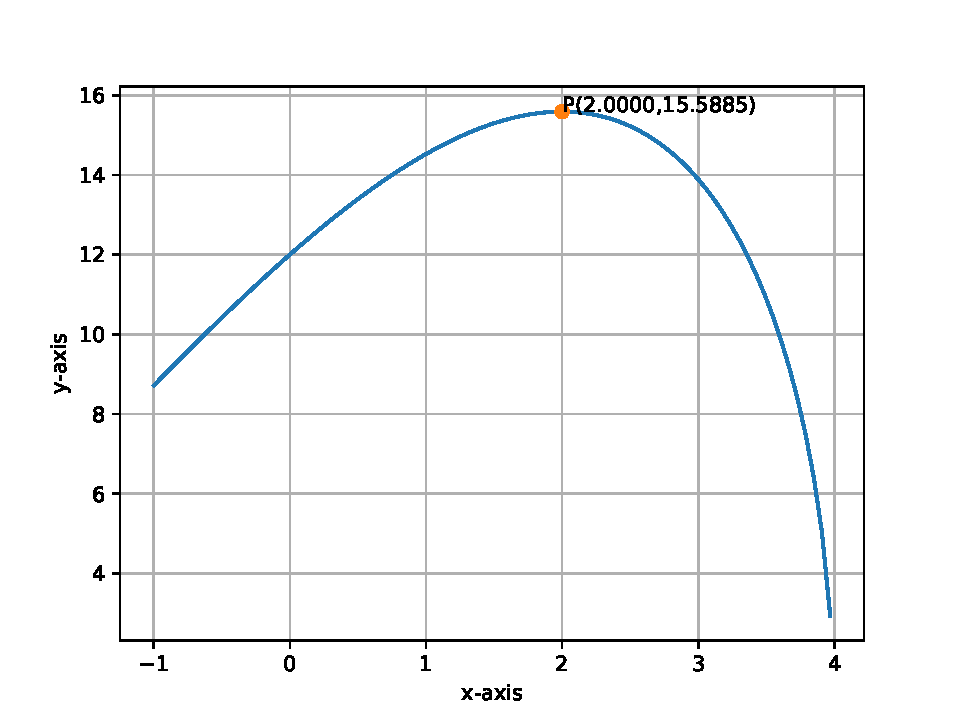
\includegraphics[width=\columnwidth]{12/12/2/1/figs/fig.pdf}
		\caption{}
		\label{fig:12/12/2/1}
  	\end{figure}
\section*{\large Solution}
\fi
Let the  mixture contain $x$ kg of food and $y$ kg of food.
\iffalse
Hence $x\geq0$ and $y\geq0$ \\
\fi
\iffalse
\begin{table}[htb]
\tiny
\resizebox{\columnwidth}{!}{
	\fi
The given information can be compiled in a table as 
	\begin{table}[!ht]
		\centering
\begin{tabular}{|c|c|c|c|}
\hline
	&Vitamin A(units/kg)&Vitamin B(units/kg)&Cost(Rs/kg)\\[5pt]
\hline
	Food P& 3&5&60\\[5pt]
\hline
	Food Q&4&2&80\\[5pt]
\hline
	Requirement(units/kg)&8&11&\\[5pt]
\hline
\end{tabular}
	\caption{}
		\label{table:12/12/2/1}
\end{table}
and 
\iffalse
\begin{align}
	P \geq 60x+80y\\
	3x + 4y \geq 8\\
	5x + 2y \geq 11
\end{align}
\fi
which can be expressed in vector form as
\begin{align}
	P = \min_{\vec{x}}\myvec{60&80}\vec{x}\\
	\myvec{3&4\\5&2}\vec{x} \succeq \myvec{8\\11}\\
	\vec{x} \succeq \vec{0}
\end{align}
Solving using cvxpy, we get
\begin{align}
	P_{min} = 159.99999999\\
	\vec{x} = \myvec{ 2.11436236 \\ 0.41422823}
\end{align}
